\documentclass[../Main.tex]{subfiles}
\begin{document}

\section{Ideas for New Alternative Games}
\label{chap:ideas}
The first part of our contribution describes, evaluates, and presents the background of six alternative game concepts invented during our prestudy work. 
In chapters \ref{chap:designanenjoyable}, \ref{chap:playertypes}, \ref{chap:rewardsystems}, we studied how to create an enjoyable game, player types, and reward systems that gave us insight on game design. In Chapter \ref{chap:what_is_alternative}, we described what an alternative game is, which helped us see the possibilities and variations within the space. By tweaking one of the six characteristics, we were able to come up with new ideas that we otherwise would not have considered. Finally, Chapter \ref{chap:existing_games} gave us an overview of existing alternative games. This research showed us examples of the current possibilities and stimulated our fantasy to invent even more ideas. The work we did in the prestudy, especially chapters \ref{chap:designanenjoyable}-\ref{chap:what_is_alternative}, will also be helpful when we choose which concept we will continue to work on.

After outlining and evaluating the six ideas, the model defined in our prestudy will be used to compare them. This comparison will help to describe the differences between the games and why they characterize as alternative games.

Our primary motivation for choosing this specific task was the opportunity to create an application with a socially beneficial purpose. The concepts should preferably introduce something valuable to society and explore the genre of alternative games. Also, the goal was to make the application available to as many users as possible. Based on these factors, we decided early that the game had to be based on the mobile platform. Consequently, the concepts described later in this chapter are invented, to various degrees, with this in mind. Over three billion people own a smartphone today \citep{odea_smartphone_2020} and the vast majority of these people use either iOS or Android \citep{statcounter_mobile_2020}. By targeting the smartphone market and these two operating systems, we can reach a lot of potential users. Besides, smartphones have a variety of sensors that can be used in alternative games.

Another important consideration that we kept in mind during the invention process was that the concept needed to be easy to test. The application’s testability is essential when we are later developing the chosen concept in our master’s thesis. We want to find out how people are using the application and whether or not they are enjoying it.

Even though these restrictions limit the possibility of concepts that can be considered, we felt it improved our ability to be creative and invent new ideas. Early on, before settling on these restrictions, the scope of alternative games was too big, making it hard to come up with anything at all.

\subsection{Hover}
\label{sec:hover}
The first alternative game idea we invented is named Hover. The concept is inspired by the existing application \textit{Hold}, described in Chapter \ref{chap:existing_games}. In short, players  get points in Hold for not using their phone. Hover uses the same principle, but the points are awarded based on their location. Meaning the players get points when they are located at certain spots in the real world. The points can then later be used to receive rewards, such as discounts or free items.

The spots are based on locations that could improve a person’s well-being, such as training centers, schools, libraries, museums, and art galleries. The locations are classified into four different categories corresponding to their purpose; health, knowledge, cultural and social. For example, training centers will be categorized as health, school as knowledge, museums and concert venues as culture, and bowling alleys and restaurants as social. The rewards and points will be summarized both for the individual categories and to a total score. In this way, the players can focus on doing their best in a specific category or try to get the best overall score. 

A crucial part of the game concept is to get people to use the application. The social interaction in the game is an important aspect to achieve that. One way of doing this is by introducing more points if a player is using the application while being together with friends. For example, if two or more players study together, they get double the amount of points. This aspect is particularly relevant in today’s situation with the COVID-19 pandemic in the world. Papers are suggesting that more people are struggling with loneliness \citep{groarke_loneliness_2020}. The application can contribute to improving mental health by motivating people to engage socially.

The game’s social aspect is also essential to increase player enjoyment in the game, as described in the GameFlow article in Chapter \ref{chap:designanenjoyable}. A highscore list where players can compare themselves against others, including their friends, is a simple way of encouraging competition. 

The game concept can be more enjoyable for the players by including elements of fantasy, as discussed by Malone (see Chapter \ref{chap:designanenjoyable}). A suggestion here is to include a virtual character that evolves depending on the number of points the player has earned during a period, e.g., the last 30 days, for the different categories. An example of how the virtual character could evolve when improving the health category is illustrated in Figure \ref{fig:player_evolement} below. 

\begin{figure}[H]
    \centering
    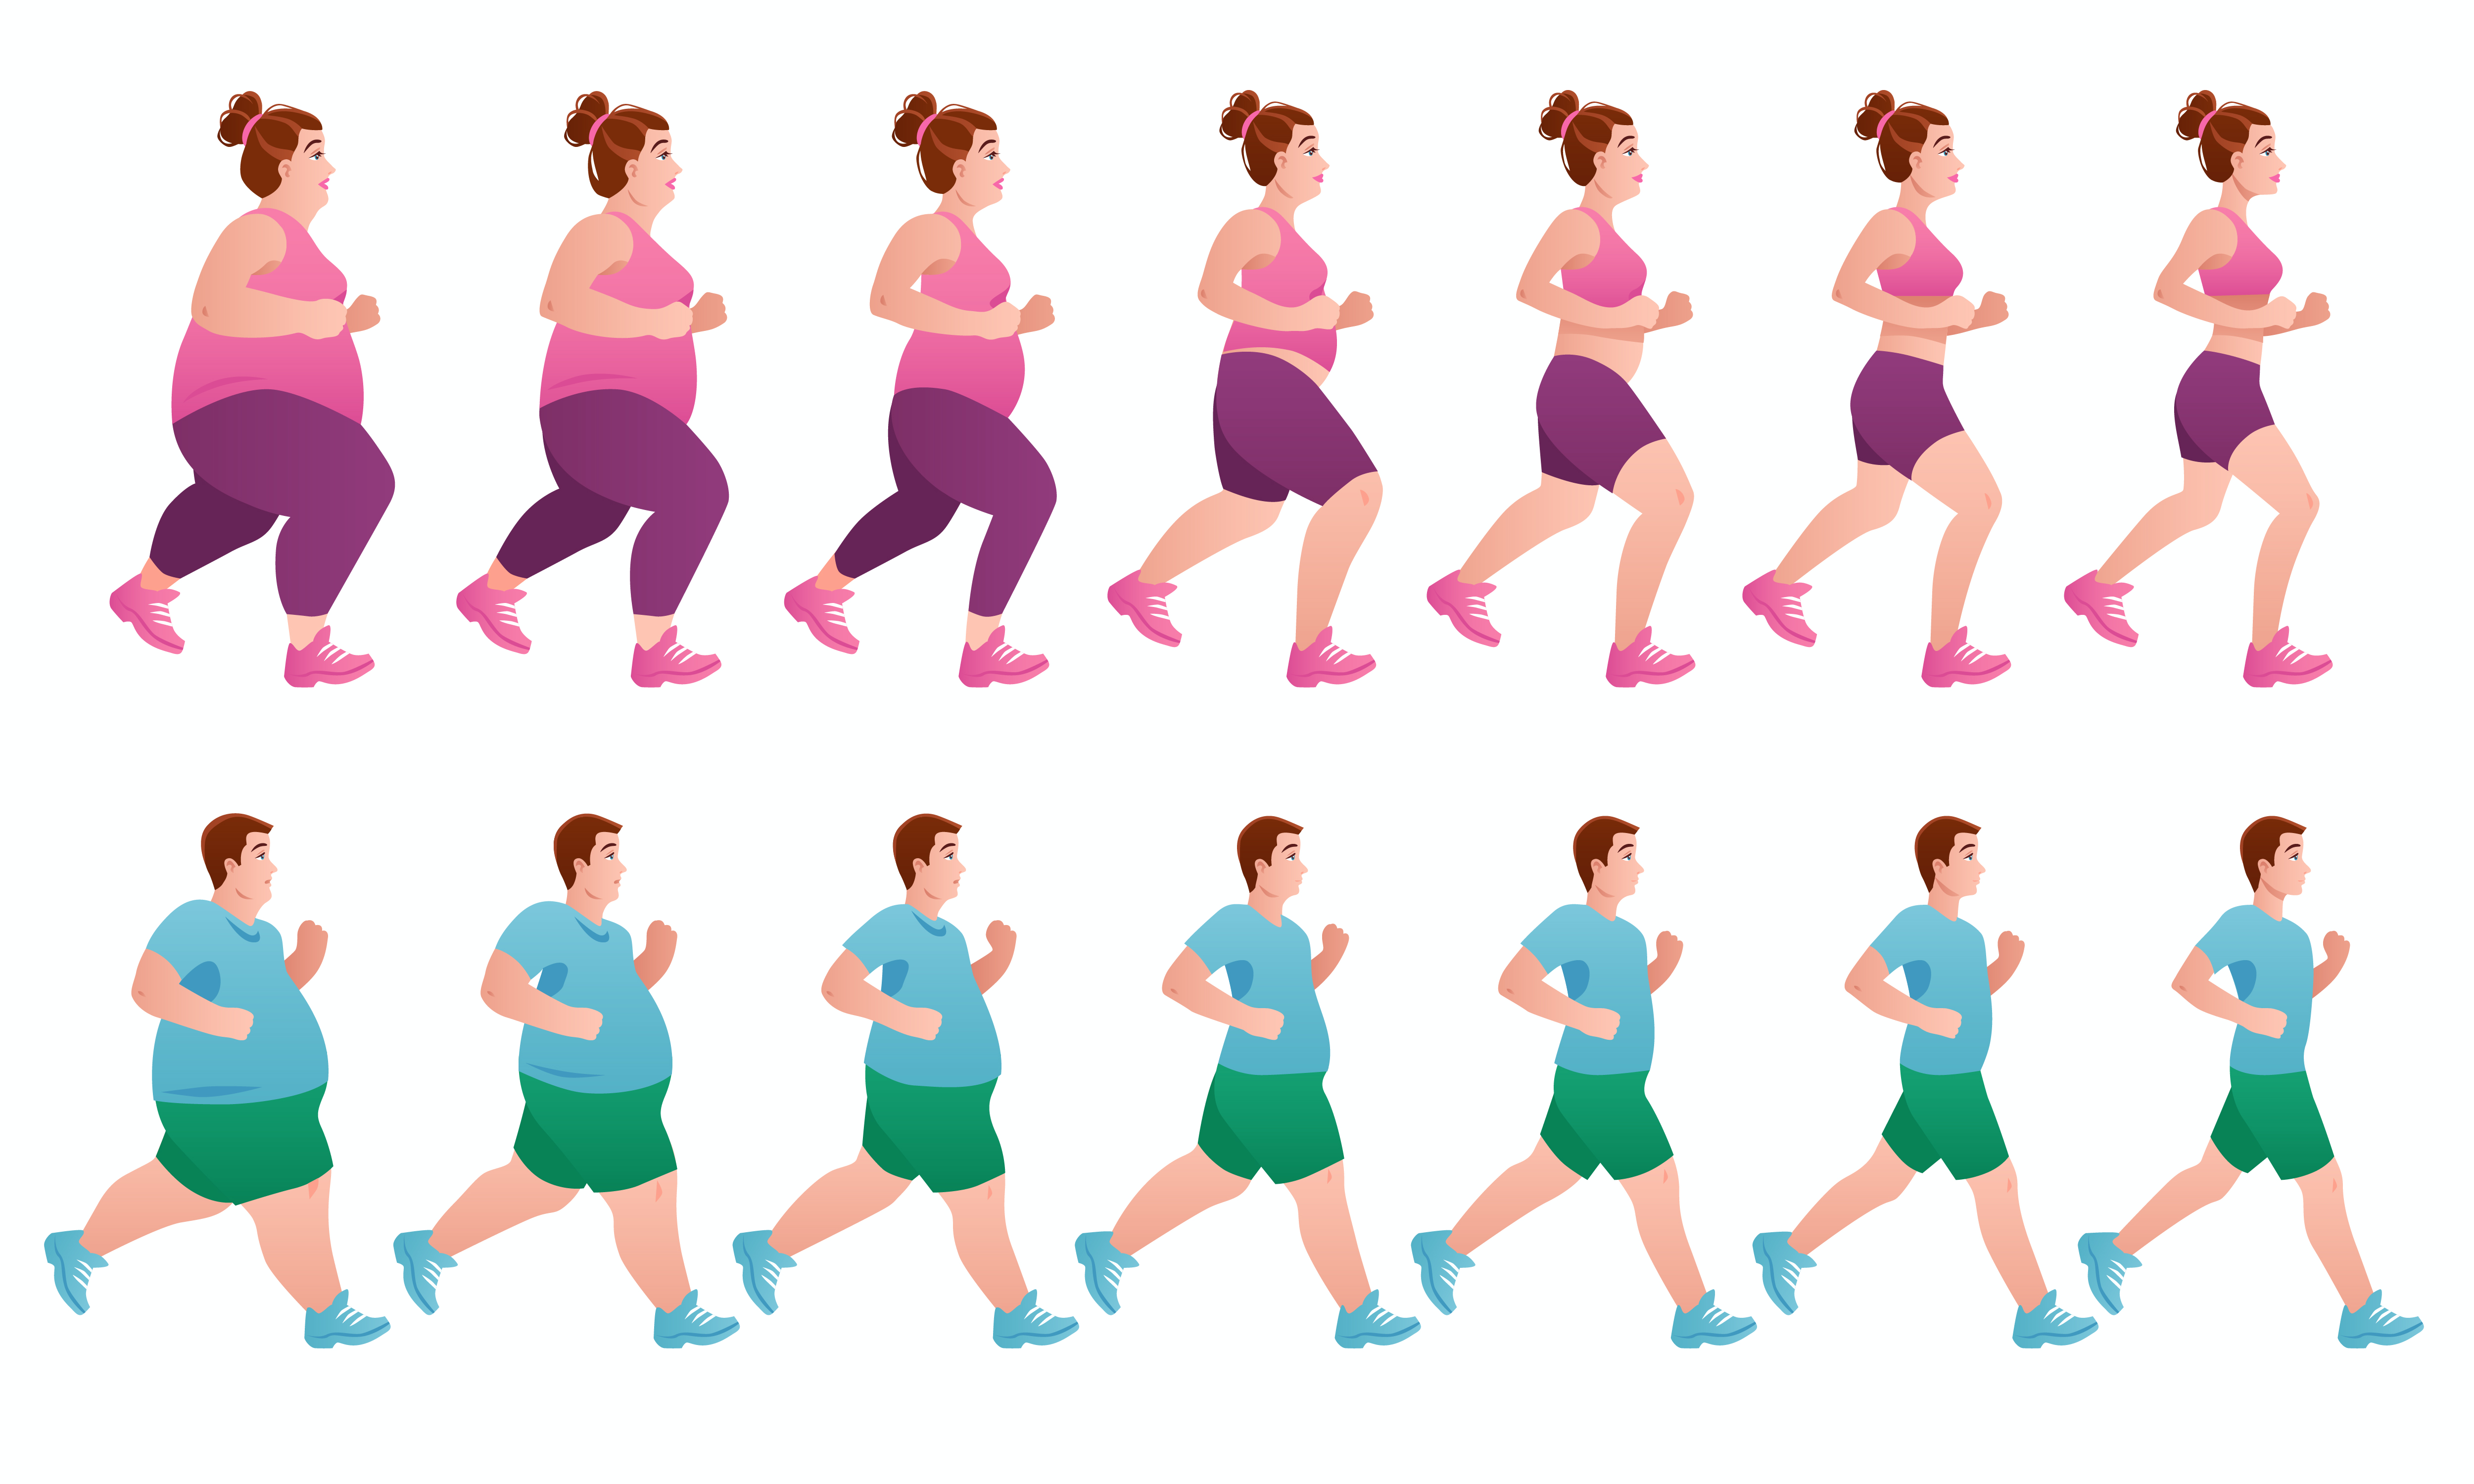
\includegraphics[width=.75\textwidth]{Images/OurConcepts/ExerciseTransformation.png}
    \caption{Example of how a virtual character could evolve in Hover.}
    \label{fig:player_evolement}
\end{figure}

To register when the players are positioned at locations where they should earn points, geofencing will be used. Geofencing is based on defining areas on the map (illustrated in Figure \ref{fig:geofence}) where one can check whether or not the user is inside \citep{rouse_what_2016}. If the GPS location corresponds to a spot within the area, the player will be awarded points. Points could then be awarded for every fifteen minutes the player stays inside the geofence.

\begin{figure}[H]
    \centering
    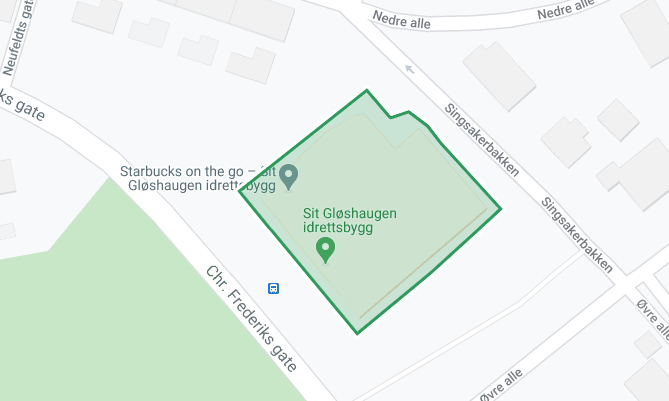
\includegraphics[width=.6\textwidth]{Images/OurConcepts/GeofenceSIT.png}
    \caption{A geofence surrounding Sit Gløshaugen training center in Trondheim.}
    \label{fig:geofence}
\end{figure}

\textbf{Evaluation} \\
Hover is, equivalent to Hold, categorized as an alternative game primarily based on two characteristics: Exploring alternative games genre by using gamification and using location data (GPS) in the gameplay.

The idea tries to increase people's well-being by motivating people to improve health, mental capabilities, socialize, and more. If the game concept is successful, it is valuable for both society and the individual.

Another important aspect when evaluating the concept is testability. Hover is easy to test because it has an unusually large target group. Everyone that owns a smartphone is a potential test subject. In addition to this, we think it will be easy to get people who agree to test this application because no extra time (despite answering a questionnaire) is required. The concept will fit almost every person.

\subsection{Guess Where}
\begin{wrapfigure}{r}{0.45\textwidth}
    \centering
    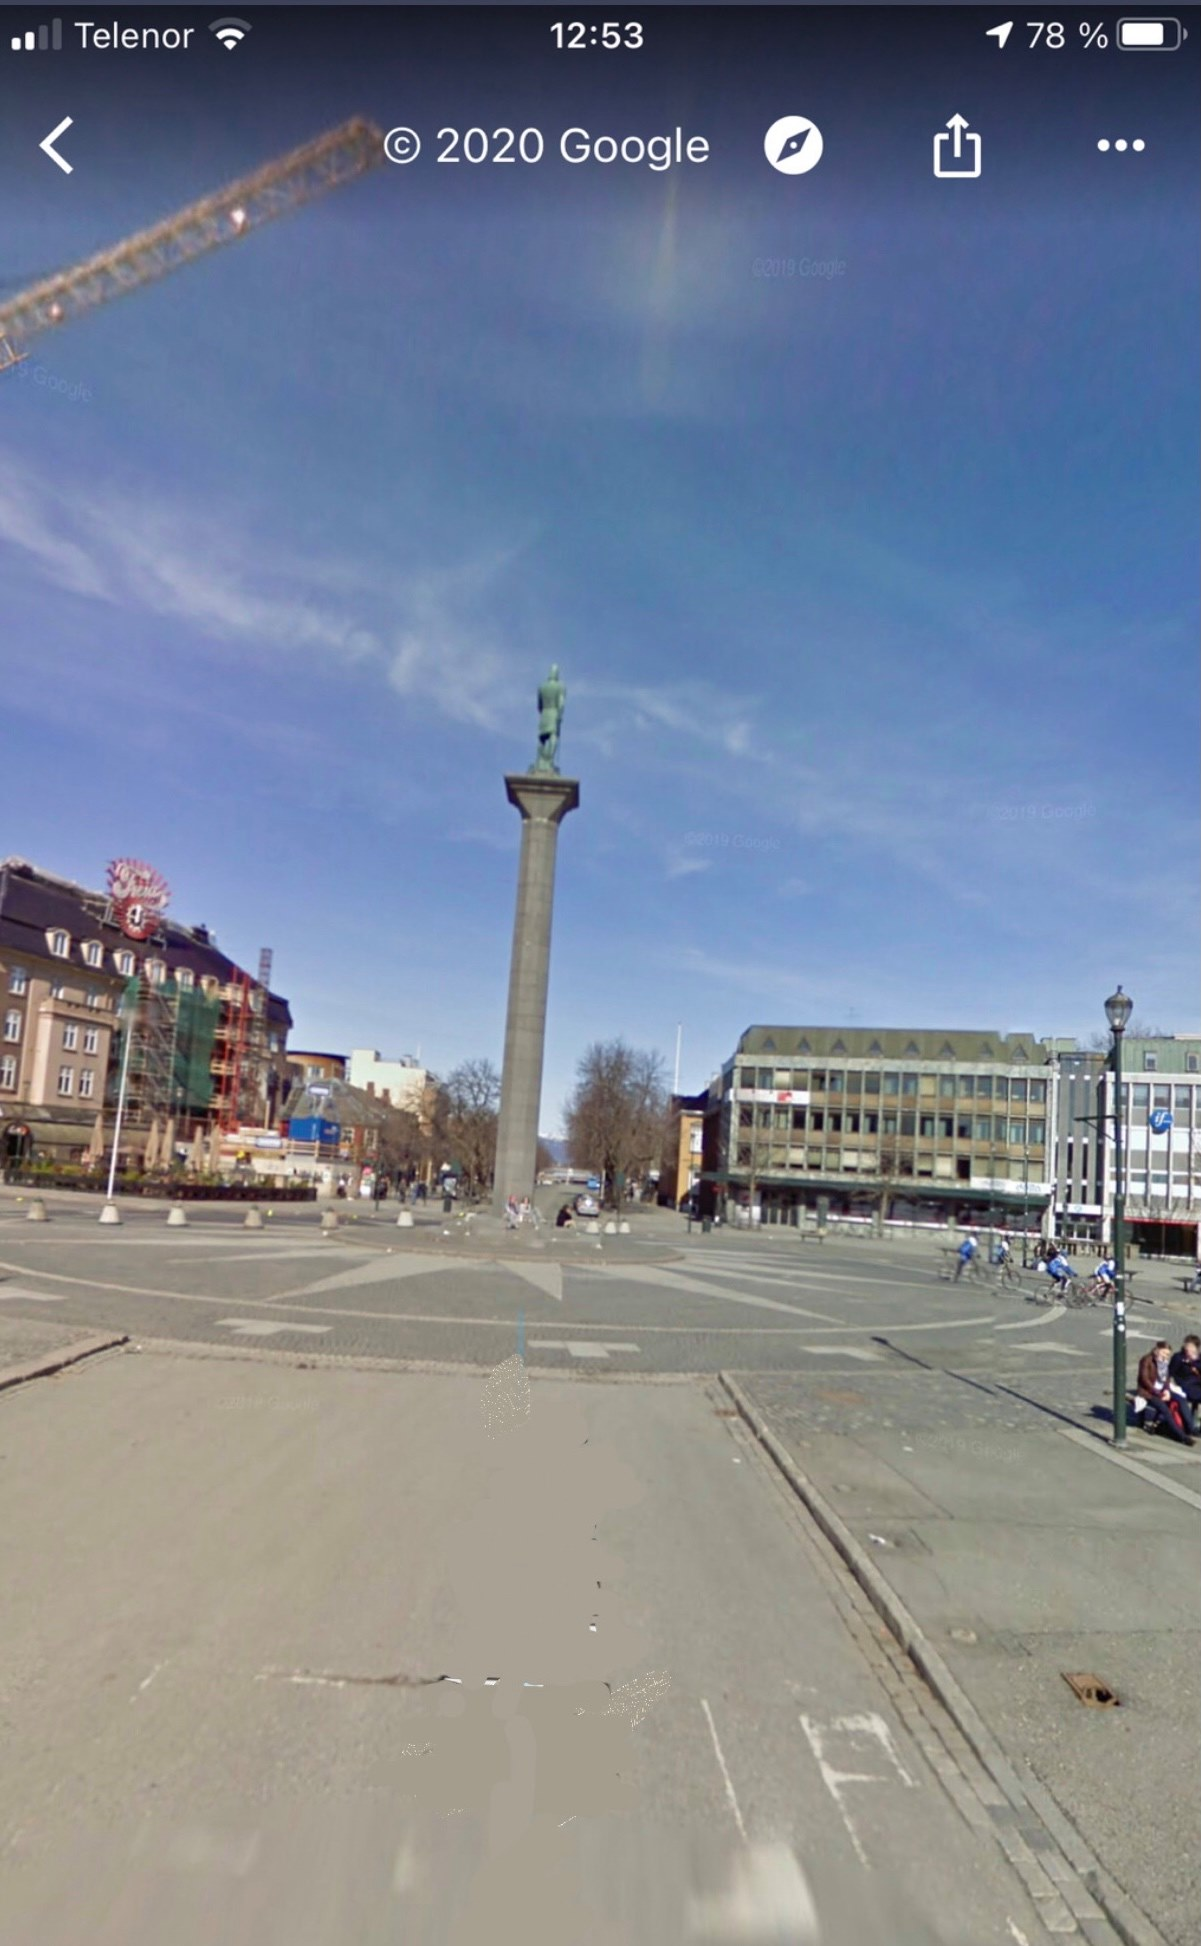
\includegraphics[width=0.35\textwidth]{Images/OurConcepts/streetView.jpg}
    \caption{A street view photo of Trondheim Torg used as a hint in Guess Where.}
    \label{fig:street_view}
\end{wrapfigure}

Guess Where is a challenge game, where players get to test how well they know their city. To earn points, players have to solve the challenges presented. A challenge consists of a street view picture where the player must figure out at which location it is captured, see Figure \ref{fig:street_view}. To complete the challenge, the players must navigate to the given location, where the challenge is verified using GPS. The game is intended to reward completed challenges with fun facts about the area and in-game points.

The concept can allow social interaction, both in the game and the real world. Players are encouraged to team up to boost their points. Accomplishments can also be shared with friends in a social feed inside the application. Social interaction through likes and comments can be motivating for further use. The concept is excellent for people that already have some knowledge of the city. However, by enabling hints, users can more easily complete the challenges. 

\textbf{Evaluation} \\
The concept fits into the alternative game model for several reasons, one being that the game is pervasive because it extends to the real world. For input, the game utilizes GPS for verifying a player’s location. In addition to this, the game fits into the domain of both entertainment and education. The game can also be categorized as the genre gamification that is considered an alternative game genre. 

The game concept is beneficial for society because it is a social game that encourages physical movement and collaboration, while players can get to know the area better. One approach is to use this game for edutainment purposes. Teenagers can team up and use this game for orientation in their gym class. This approach is not only beneficial for the sake of moving around in the city, but teenagers can also improve their cooperation skills. In terms of testability, this concept could, for instance, be tested in a high school class.

During the process of inventing new game concepts, we discovered the article called “A pervasive game to get to know your city better” by \citeauthor{wang_pervasive_2011} (\citeyear{wang_pervasive_2011}). The article presents a game called “The Amazing City Game” (ACG), which focuses on finding certain spots in the city based on clues. 

Though the game concepts have a lot in common in terms of physical movement, real-world social interactions, and triggering player curiosity, there are some differences. Mainly that ACG has more focus on competing against other teams, whereas Guess Where concentrates on social interaction from sharing accomplishments.

\subsection{Puzzle with Friends}
Puzzle with Friends is a game concept where the goal is to complete a puzzle together with your friends, as illustrated in Figure \ref{fig:friends_puzzle}. Each player is responsible for one piece they can move using their real-world position, and by rotating the mobile phone. All participants can watch the other players’ positions and the pattern they are supposed to puzzle in the application. The goal is to complete the puzzle, fit all the pieces in the correct spot, and rotate them correctly before the time is up. The number of pieces depends on how many players collaborating on the same puzzle. If eight friends are trying to solve a puzzle, there will be eight pieces, and so on. Thus the game will become increasingly challenging as the number of players increases. For the game to not become too easy, there should be a limitation on the minimum amount of players.

\begin{figure}[H]
    \centering
    \includegraphics[width=0.7\textwidth]{Images/OurConcepts/teamwork_puzzle.jpg}
    \caption{People trying to solve puzzle, illustrating the concept in Friends Puzzle}
    \label{fig:friends_puzzle}
\end{figure}

\begin{wrapfigure}{r}{0.4\textwidth}
    \centering
    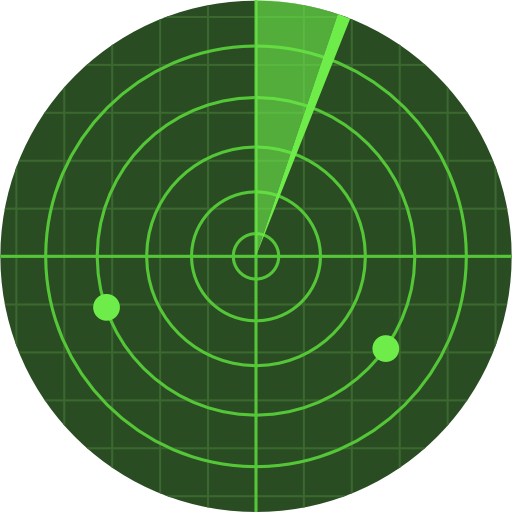
\includegraphics[width=0.35\textwidth]{Images/OurConcepts/radar.png}
    \caption{A typical radar view. The “dots” will update every time the beam passes by.}
    \label{fig:radar_view}
    \vspace*{-1\baselineskip}
\end{wrapfigure}

GPS location will be used to determine the player’s position. Because of the limitation in GPS accuracy \citep{merry_smartphone_2019}, a large outdoor area is required for the game to work as intended. Parks or football fields are good examples. Also, the more players that are included in the game, the more space is needed. Hence, there probably should exist a maximum number of players per game. The gameplay should also include a suitable mechanism for “snapping” pieces into the correct place when they are almost correctly aligned. This tool will make the game more delightful to play when minor location errors are present.

As there probably will be some delay between the player’s movement and the application’s view, the gameplay needs to introduce some mechanism to hide this. One way to do this is by introducing some sort of radar view, see Figure \ref{fig:radar_view}, to illustrate that the other players’ position will only update at regular time intervals. 

\textbf{Evaluation} \\
Puzzle with Friends is a typical alternative game because it uses alternative inputs to create a unique game concept. By utilizing the player’s position and heading in the real world to control the gameplay, the game is differentiated from other well-known puzzle games.

Developing the game should be manageable in the limited time we have during our master’s project. However, as mentioned above, inaccurate location data and real-time requirements may cause issues if not handled appropriately. Testing the application should be easy as long as we find some volunteers who agree to devote some hours of their day for testing the application. 

\subsection{Challenge Accepted}
\begin{wrapfigure}{r}{0.45\textwidth}
    \vspace*{-1\baselineskip}
    \centering
    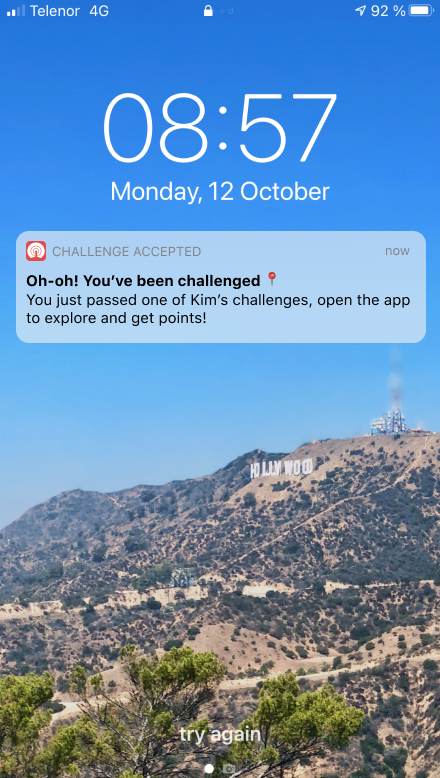
\includegraphics[width=0.30\textwidth]{Images/OurConcepts/ChallengeAcceptedNotification.png}
    \caption{Example of push notification in Challenge Accepted.}
    \vspace*{-2\baselineskip}
    \label{fig:challenge_accepted_notification}
\end{wrapfigure}

Challenge Accepted is a social game that mixes social interaction with playful actions in the real world. The idea is based on a verbal game, often played among youths, called \href{https://www.wikihow.com/Play-What-Are-the-Odds}{"What are the odds?}". The game is usually played between two players where one player (A) gives the dare, and another player (B) receives it. The challenges often occur in the moment, for instance, “What are the odds of you asking that stranger to try his crutches?” To extend the concept a bit, players can publish challenges on a location that pops up when their friends walk by.

\begin{figure}[H]
    \centering
    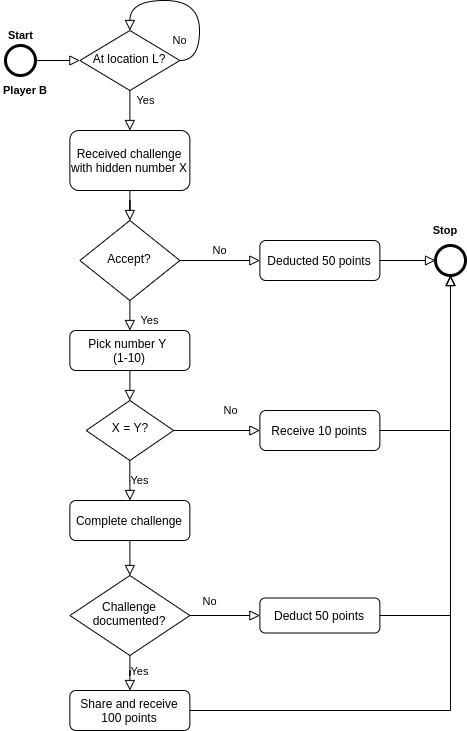
\includegraphics[width=.5\textwidth]{Images/OurConcepts/ChallengeAccepted.png}
    \caption{Flow chart illustrating a simplified game flow in Challenge Accepted.}
    \label{fig:challenge_accepted}
\end{figure}

Figure \ref{fig:challenge_accepted} shows a simplified diagram of the game flow. The diagram is based on the following scenario:

\begin{itemize}
    \item Player A adds a challenge to a location L, along with a number X between 1 and 10.
    \item A friend of player A, player B, walks by the location and receives a push notification, as seen in Figure \ref{fig:challenge_accepted_notification}.
    \item Player B has to either decline or accept the challenge. If the player chooses to decline, 50 points are lost. If the challenge is accepted, player B has to guess a number between 1 and 10.
    \item If the numbers are different, the player will not need to complete the challenge and receive 10 points for being courageous.
    \item However, if the numbers are equal, player B needs to do it. The challenge is considered completed when it is documented and shared in the application.
\end{itemize}

The goal of the game is to create spontaneous and surprising enjoyment between friends. The range is set between 1-10 because the risk of having to complete a challenge should not be too high nor too low. Also, challenges should be moderated to prevent them from being harmful. The game should include social interaction through likes and comments on in-game posts. Players should also be able to see their friends' game statistics and medals. This can likely have a positive effect on the competitiveness among friends.

\textbf{Evaluation} \\
The concept classifies as alternative in the categories of input, game genre, and interaction. Besides location tracking, the concept also utilizes the camera for documenting challenges. Though the game is based on a verbal game, the game categorizes as gamification, because players can be motivated through likes and comments on recent activities. 

The game is a pervasive game that utilizes location-tracking to create a bond between the virtual world and the real world. The use of constant tracking of location contributes to the suspense of not knowing when, where and what the next challenge will be. This suspense can also increase the players’ curiosity, and therefore willingness to participate. 

The concept does not necessarily benefit society directly, however it is a social game that has value for a smaller group of people. For testing purposes, it is advantageous to test the game on people that have a pre-existing relationship. This is because the game uses this relation within the frame of the game to enhance emotions that motivate the player to complete the challenges.

\subsection{Secret Posts}
Secret Posts is an extension and gamification concept based on the social app Jodel, where users can share anonymous posts in their city. Since the posts are anonymous, people tend to post their secrets, embarrassing stories, and pictures. Our concept involves posting digital notes, drawings, or images in the real world, which only can be seen using Augmented Reality (AR) technology. All users can share posts attached to the location where they are posted. An example can be a sticky-note with a secret message laying on a table in a cafeteria. To find posts players use a map to locate nearby ones, as seen in Figure \ref{fig:secret_notes_map}. Although the location of the posts is visible on the map, the content is only available through the mobile camera. As illustrated in Figure \ref{fig:secret_notes_camera}, players use their mobile camera to read new posts in their current area. When a user finds a post, he or she can choose to save it. Since the posts only are visible to the players, a secret society is created where only those who know, know.

Besides the example views in Figure \ref{fig:secret_notes_map} and Figure \ref{fig:secret_notes_camera}, the application should also have a view for posting at the current location, and a view for saved and own posts.

\begin{figure}[H]
    \begin{minipage}{.48\textwidth}
        \centering
        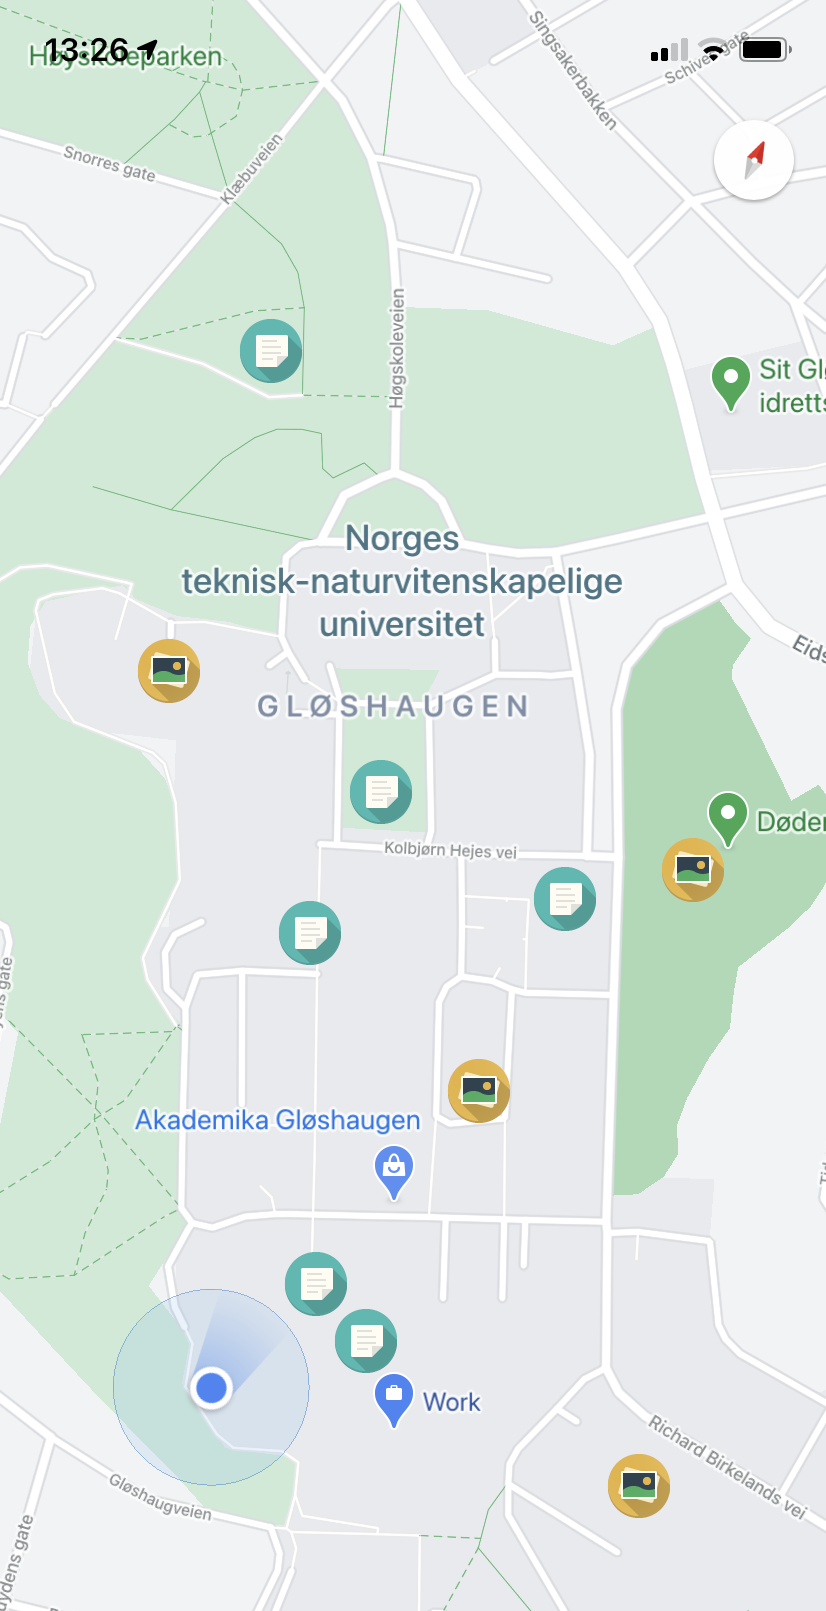
\includegraphics[width=.8\textwidth]{Images/OurConcepts/secret_notes_map.png}
        \captionof{figure}{The map-view in Secret Notes showing nearby posts.}
        \label{fig:secret_notes_map}
        \end{minipage}
        \hspace*{0.5\baselineskip}
        \begin{minipage}{.48\textwidth}
        \centering
        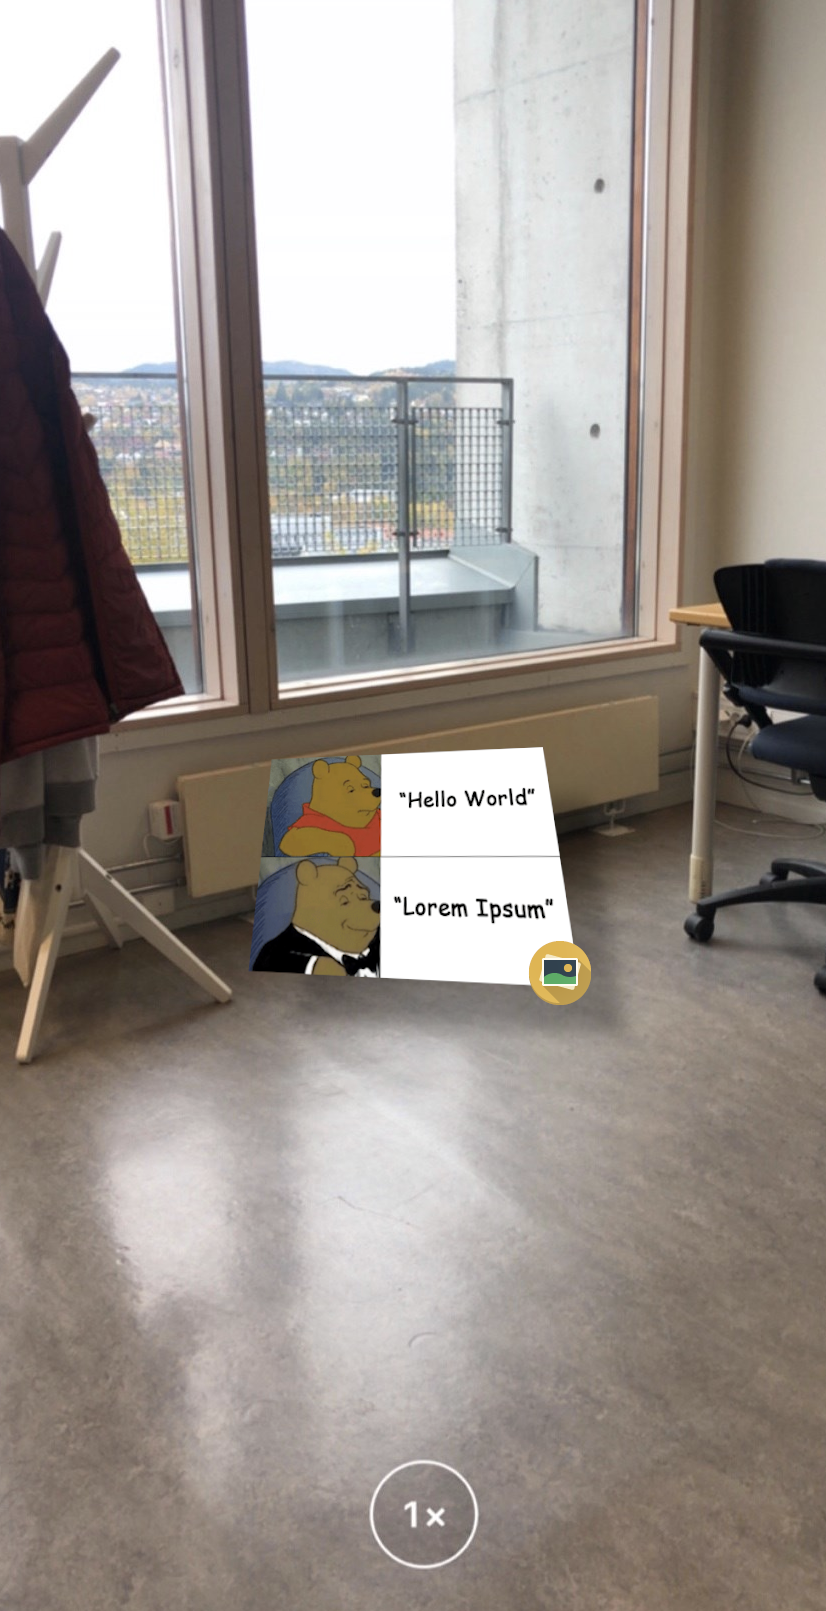
\includegraphics[width=.8\textwidth]{Images/OurConcepts/secret_notes_camera.png}
        \captionof{figure}{AR view of the content of a note found in Secret Notes.}
        \label{fig:secret_notes_camera}
    \end{minipage}
\end{figure}

\textbf{Evaluation} \\
The concept is alternative in its usage of input, output, game genre, and concept. The game uses the phone’s camera for input, which it uses to project a note, image, or drawing. This usage of AR is not too common as of 2020, hence the input method is alternative. The concept is also alternative because it uses location to attach anonymous posts. Tangible objects like notes, posters, and graffiti are not unfamiliar in the real world. However, the fact that the posts are only visible for those who search, makes the game concept alternative.

The concept is suited for AR glasses and as a mobile application. The benefit of using AR glasses is that the users can walk around and discover notes without actively looking. However, in terms of testability, the AR approach has a clear disadvantage compared to a mobile application in terms of equipment available and the time scope of the project. As a mobile application, the concept is easy to develop and test. However, the technology will most likely struggle to distinguish location properly when the user is located inside a building \citep{xia_using_2015}. Distinguishing location on the vertical axis in three-dimensional space is very hard to include in a mobile application. For instance, a post that is posted on the third floor of a building will be readable for every floor in that location. As a consequence of this, the application may work best outside, and a solution could be to only allow posts outside. But this removes some of the excitement and mystery of the concept.

\subsection{Free Ticket to Ride}
The purpose of this game concept is to incentivize having a valid ticket when using public transport. The idea is to create an application that gamifies the ticket system used on public transport. It could be adopted as an alternative or addition to regular ticket controls used today.

The application will need to integrate with the existing ticket application to validate tickets. People who have paid for a valid ticket will be given points in the game when they are traveling. After earning a set amount of points, the user can “purchase” free items or get discounts. One suggestion is to use free or discounted single tickets as rewards. For example, twenty rides with a valid ticket could qualify for one free ticket. A prerequisite for this is of course a partnership with a public transport company, such as AtB in Trondheim. Even though the concept is invented and conceptualized based on the public transport system in Trondheim, the same ideas could be adopted in other cities with similar ticket systems as well.

To register valid rides, the application will use Bluetooth. The user’s smartphone communicates with a Bluetooth access point to register when the user is located in a public transport vehicle (illustrated in Figure \ref{fig:people_on_the_bus}). The application will then check if the ticket is valid and award the user points if that is the case. The smartphone camera could also be used as a secondary registration option, by scanning QR-codes to get points. This could be an alternative to situations where the user does not want to consent to Bluetooth usage.

\begin{figure}[H]
    \centering
    
\includegraphics[width=0.75\textwidth]{Images/OurConcepts/PeopleOnTheBus.png}
    \caption{Illustration of people using Free Ticket to Ride on public transport.}
    \label{fig:people_on_the_bus}
\end{figure}

\textbf{Evaluation} \\
Free ticket to ride is an alternative game concept because it uses Bluetooth for input. Additionally, as mentioned above, the concept explores the gamification genre. By the definition of what an alternative game is in Chapter \ref{chap:what_is_alternative} these two characteristics define this an alternative game.

The game introduces a fun way of validating the user’s ticket when using public transport, which in turn could lead to fewer fare evasions. Getting more people to pay for their ride will result in more income for the public transport company, which can be used on improving the service.

One of the main problems with this idea is the need for tight integration with the current public transport company. The concept requires integration with the ticket system to check the validity of the ticket. Additionally, this idea requires a hardware Bluetooth device mounted on every bus, to check that the user is traveling. 

\subsection{Comparison of Game Concepts}
Similarly as in Chapter \ref{chap:existing_games} and Chapter \ref{chap:comparison_of_existing}, when existing alternative game concepts were presented, our new ideas are compared using the alternative games model presented in Chapter \ref{chap:what_is_alternative}. All of the game concepts are categorized using the six characteristics of alternative games.

\begin{table}[H]
    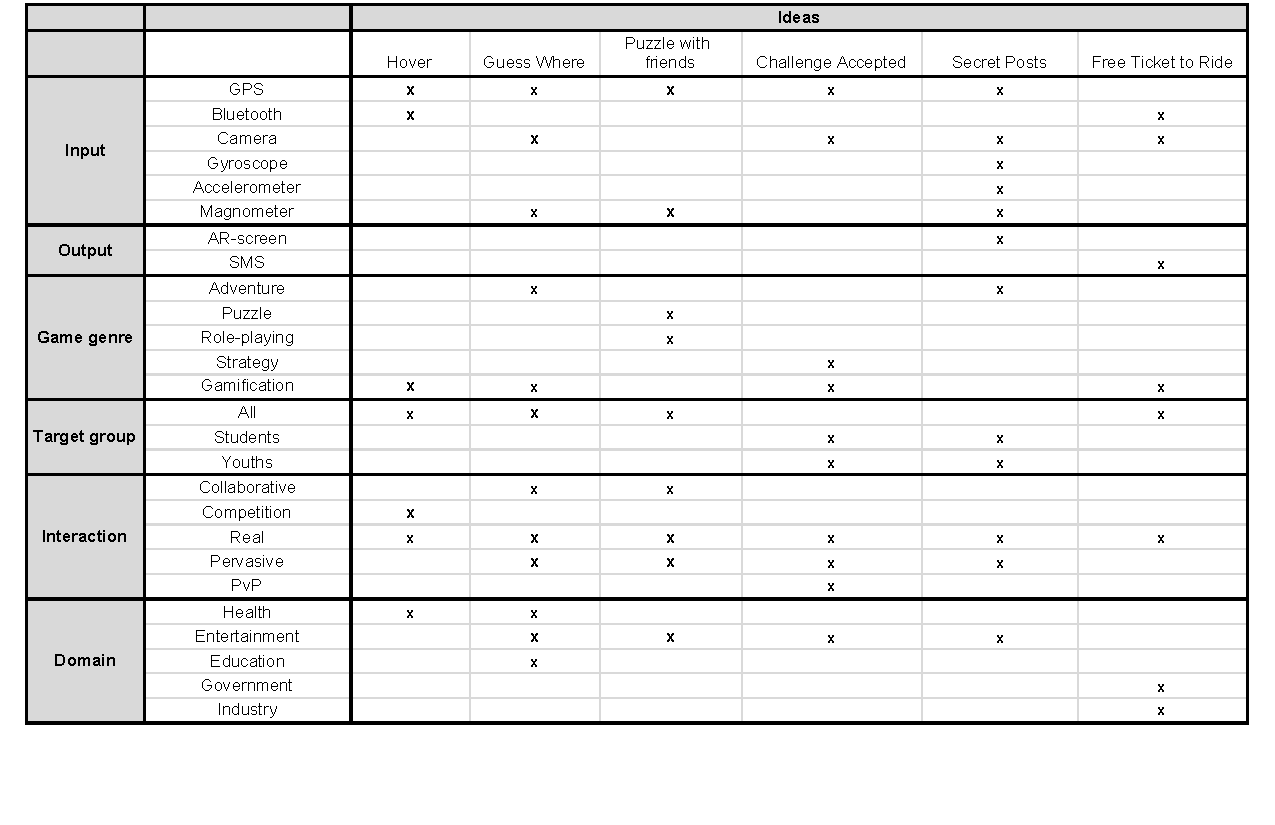
\includegraphics[width=1\textwidth]{Images/Models/OurConcepts.pdf}
    \vspace*{-3\baselineskip}
    \caption{Our concepts alternative games characteristics}
    \label{tab:our_concepts}
\end{table}

In contrast to the comparison of existing alternative games, our new concepts have a lot in common, and often tick the same boxes in the model, as seen in Table \ref{tab:our_concepts}. The existing alternative games were picked partly based on their difference, so this is expected. As mentioned at the beginning of this chapter, we limited ourselves to concepts based on the mobile platform. Thus all the games are restricted to input and output provided by a smartphone. For input, a selection of the available sensors have been used in our ideas, where some of these have been used more frequently than others. GPS for location tracking is the most common input sensor with four out of six concepts using it. Output possibilities on a mobile phone are more limited. There are not a lot of possible outputs that we would categorize as alternative. Two exceptions are found in Mysterious Posts and Free Ticket to Ride. These games respectively use an AR screen for displaying the notes and SMS to verify users and notify them of important events, respectively.

One of the most notable similarities in our new concepts is the use of gamification as the game genre. The reason for this is related to our goal in the project; trying to do something socially beneficial. We found it easier to come up with gamification concepts with socially beneficial purposes than real game concepts.

As we also described in the background, an important factor when inventing ideas was to try to reach as many users as possible. Therefore, the applications are usually targeted to all user types. However, two of the ideas have youths and students as the main target group. This does not mean that adults cannot use them, it is only this group of people the games are primarily made for. 

The last two categories address interaction and domain. In the interaction category, we see that all games include aspects of the real-world. Four of the games are also pervasive, meaning that they mix reality and virtuality. The most common domain in the applications is entertainment with four of six applications characterized as it. Hover and Free Ticket to Ride are the only ones that are not categorized as entertainment. They fall into the health and government/industry domain respectively.

\subsection{Summary}
In this chapter, our ideas for new alternative game concepts were described. A brief description of all of the concepts and an evaluation of them was conducted. We looked at why the concepts can be categorized as alternative games and how they fit with our goal and motivation in the project. Additionally, we looked at the testability of the ideas. Last, we compared the concepts and looked at differences using the alternative games model defined earlier. The next chapter will use these observations and evaluations when we will choose the concept which we are going to develop in our master’s thesis.

\biblio % Needed for referencing to working when compiling individual subfiles - Do not remove
\end{document}